\documentclass[12pt,tikz]{standalone}

\usepackage[utf8]{inputenc} % use UTF-8
\usepackage{mmap}
\usepackage[T2A,OT1]{fontenc} % rus fonts
\usepackage[russian]{babel} % russian language

\usepackage{tkz-euclide}
\usetikzlibrary{shapes,backgrounds}

\tikzstyle{startstop} = [rectangle, rounded corners, minimum width=3cm, minimum height=1cm,text centered, draw=black, fill=red!30]

\tikzstyle{io} = [trapezium, trapezium left angle=70, trapezium right angle=110, minimum width=3cm, minimum height=1cm, text centered, draw=black, fill=blue!30]

\tikzstyle{process} = [rectangle, minimum width=3cm, minimum height=1cm, text centered, draw=black, fill=orange!30]

\tikzstyle{decision} = [diamond, minimum width=3cm, minimum height=1cm, text centered, draw=black, fill=green!30]

\tikzstyle{arrow} = [thick,->,>=stealth]
 
\begin{document}
		\begin{tikzpicture}[node distance=4cm]
		\node[anchor=south west,inner sep=0] (gui) at (0,0) {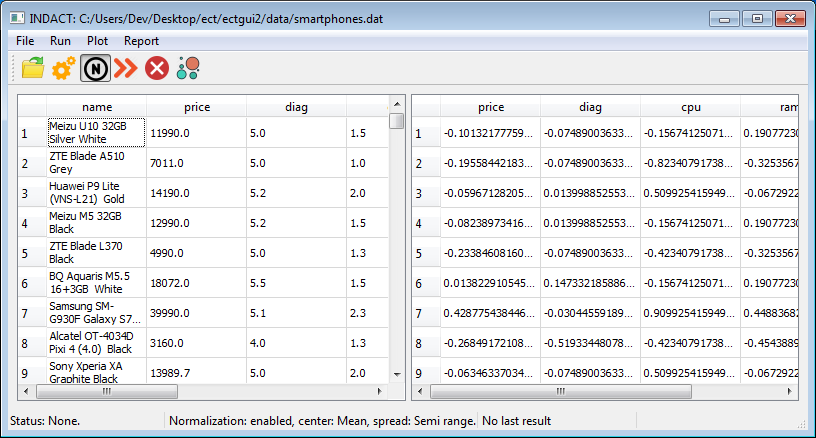
\includegraphics{/home/eremeykin/d_disk/ereme/GoogleDrive/HSE/Diploma/tex/img/main-gui.png}};
		
		\draw[draw=black, fill=green!50, fill opacity=0.2, shift={(0,0)}, dash pattern=on 3pt off 3pt] (0.3,0.8) rectangle ++(10.5,8.4);
		
		\draw[draw=black, fill=blue!50, fill opacity=0.2, shift={(0,0)}, dash pattern=on 3pt off 3pt] (10.8,0.8) rectangle ++(10.5,8.4);
		
		\draw[fill=white] (5.5,5.5) circle (0.3);
		\node[text=black] at (5.5,5.5) {3};
		
		\draw[fill=white] (16.5,5.5) circle (0.3);
		\node[text=black] at (16.5,5.5) {4};	
		
		\draw[fill=white] (6.2,9.8) circle (0.3);
		\node[text=black] at (6.2,9.8) {2};
		
		\draw[fill=white] (5,10.53) circle (0.3);
		\node[text=black] at (5,10.53) {1};
		
%		\tkzInit[xmax=16,ymax=11,xmin=0,ymin=0]
%					\begin{scope}[dash pattern=on 1pt off 4pt]
%					\tkzGrid
%					\end{scope}
%		\tkzLabelX[orig=true,label options={font=\normalfont},step=1]
%		\tkzLabelY[orig=false,label options={font=\normalfont}]
%		\tkzDrawX[label={}] %right space=1.0,
%		\tkzDrawY[label={}]	
				
		\end{tikzpicture}
\end{document}